% Options for packages loaded elsewhere
% Options for packages loaded elsewhere
\PassOptionsToPackage{unicode}{hyperref}
\PassOptionsToPackage{hyphens}{url}
%
\documentclass[
  ignorenonframetext,
  aspectratio=169,
  spanish,
]{beamer}
\newif\ifbibliography
\usepackage{pgfpages}
\setbeamertemplate{caption}[numbered]
\setbeamertemplate{caption label separator}{: }
\setbeamercolor{caption name}{fg=normal text.fg}
\beamertemplatenavigationsymbolshorizontal
% remove section numbering
\setbeamertemplate{part page}{
  \centering
  \begin{beamercolorbox}[sep=16pt,center]{part title}
    \usebeamerfont{part title}\insertpart\par
  \end{beamercolorbox}
}
\setbeamertemplate{section page}{
  \centering
  \begin{beamercolorbox}[sep=12pt,center]{section title}
    \usebeamerfont{section title}\insertsection\par
  \end{beamercolorbox}
}
\setbeamertemplate{subsection page}{
  \centering
  \begin{beamercolorbox}[sep=8pt,center]{subsection title}
    \usebeamerfont{subsection title}\insertsubsection\par
  \end{beamercolorbox}
}
% Prevent slide breaks in the middle of a paragraph
\widowpenalties 1 10000
\raggedbottom
\AtBeginPart{
  \frame{\partpage}
}
\AtBeginSection{
  \ifbibliography
  \else
    \frame{\sectionpage}
  \fi
}
\AtBeginSubsection{
  \frame{\subsectionpage}
}
\usepackage{iftex}
\ifPDFTeX
  \usepackage[T1]{fontenc}
  \usepackage[utf8]{inputenc}
  \usepackage{textcomp} % provide euro and other symbols
\else % if luatex or xetex
  \usepackage{unicode-math} % this also loads fontspec
  \defaultfontfeatures{Scale=MatchLowercase}
  \defaultfontfeatures[\rmfamily]{Ligatures=TeX,Scale=1}
\fi
\usepackage{lmodern}

\usetheme[]{default}
\usefonttheme[]{default}
\ifPDFTeX\else
  % xetex/luatex font selection
\fi
% Use upquote if available, for straight quotes in verbatim environments
\IfFileExists{upquote.sty}{\usepackage{upquote}}{}
\IfFileExists{microtype.sty}{% use microtype if available
  \usepackage[]{microtype}
  \UseMicrotypeSet[protrusion]{basicmath} % disable protrusion for tt fonts
}{}
\makeatletter
\@ifundefined{KOMAClassName}{% if non-KOMA class
  \IfFileExists{parskip.sty}{%
    \usepackage{parskip}
  }{% else
    \setlength{\parindent}{0pt}
    \setlength{\parskip}{6pt plus 2pt minus 1pt}}
}{% if KOMA class
  \KOMAoptions{parskip=half}}
\makeatother

\usepackage{color}
\usepackage{fancyvrb}
\newcommand{\VerbBar}{|}
\newcommand{\VERB}{\Verb[commandchars=\\\{\}]}
\DefineVerbatimEnvironment{Highlighting}{Verbatim}{commandchars=\\\{\}}
% Add ',fontsize=\small' for more characters per line
\usepackage{framed}
\definecolor{shadecolor}{RGB}{241,243,245}
\newenvironment{Shaded}{\begin{snugshade}}{\end{snugshade}}
\newcommand{\AlertTok}[1]{\textcolor[rgb]{0.68,0.00,0.00}{#1}}
\newcommand{\AnnotationTok}[1]{\textcolor[rgb]{0.37,0.37,0.37}{#1}}
\newcommand{\AttributeTok}[1]{\textcolor[rgb]{0.40,0.45,0.13}{#1}}
\newcommand{\BaseNTok}[1]{\textcolor[rgb]{0.68,0.00,0.00}{#1}}
\newcommand{\BuiltInTok}[1]{\textcolor[rgb]{0.00,0.23,0.31}{#1}}
\newcommand{\CharTok}[1]{\textcolor[rgb]{0.13,0.47,0.30}{#1}}
\newcommand{\CommentTok}[1]{\textcolor[rgb]{0.37,0.37,0.37}{#1}}
\newcommand{\CommentVarTok}[1]{\textcolor[rgb]{0.37,0.37,0.37}{\textit{#1}}}
\newcommand{\ConstantTok}[1]{\textcolor[rgb]{0.56,0.35,0.01}{#1}}
\newcommand{\ControlFlowTok}[1]{\textcolor[rgb]{0.00,0.23,0.31}{\textbf{#1}}}
\newcommand{\DataTypeTok}[1]{\textcolor[rgb]{0.68,0.00,0.00}{#1}}
\newcommand{\DecValTok}[1]{\textcolor[rgb]{0.68,0.00,0.00}{#1}}
\newcommand{\DocumentationTok}[1]{\textcolor[rgb]{0.37,0.37,0.37}{\textit{#1}}}
\newcommand{\ErrorTok}[1]{\textcolor[rgb]{0.68,0.00,0.00}{#1}}
\newcommand{\ExtensionTok}[1]{\textcolor[rgb]{0.00,0.23,0.31}{#1}}
\newcommand{\FloatTok}[1]{\textcolor[rgb]{0.68,0.00,0.00}{#1}}
\newcommand{\FunctionTok}[1]{\textcolor[rgb]{0.28,0.35,0.67}{#1}}
\newcommand{\ImportTok}[1]{\textcolor[rgb]{0.00,0.46,0.62}{#1}}
\newcommand{\InformationTok}[1]{\textcolor[rgb]{0.37,0.37,0.37}{#1}}
\newcommand{\KeywordTok}[1]{\textcolor[rgb]{0.00,0.23,0.31}{\textbf{#1}}}
\newcommand{\NormalTok}[1]{\textcolor[rgb]{0.00,0.23,0.31}{#1}}
\newcommand{\OperatorTok}[1]{\textcolor[rgb]{0.37,0.37,0.37}{#1}}
\newcommand{\OtherTok}[1]{\textcolor[rgb]{0.00,0.23,0.31}{#1}}
\newcommand{\PreprocessorTok}[1]{\textcolor[rgb]{0.68,0.00,0.00}{#1}}
\newcommand{\RegionMarkerTok}[1]{\textcolor[rgb]{0.00,0.23,0.31}{#1}}
\newcommand{\SpecialCharTok}[1]{\textcolor[rgb]{0.37,0.37,0.37}{#1}}
\newcommand{\SpecialStringTok}[1]{\textcolor[rgb]{0.13,0.47,0.30}{#1}}
\newcommand{\StringTok}[1]{\textcolor[rgb]{0.13,0.47,0.30}{#1}}
\newcommand{\VariableTok}[1]{\textcolor[rgb]{0.07,0.07,0.07}{#1}}
\newcommand{\VerbatimStringTok}[1]{\textcolor[rgb]{0.13,0.47,0.30}{#1}}
\newcommand{\WarningTok}[1]{\textcolor[rgb]{0.37,0.37,0.37}{\textit{#1}}}

\usepackage{longtable,booktabs,array}
\usepackage{calc} % for calculating minipage widths
\usepackage{caption}
% Make caption package work with longtable
\makeatletter
\def\fnum@table{\tablename~\thetable}
\makeatother
\usepackage{graphicx}
\makeatletter
\newsavebox\pandoc@box
\newcommand*\pandocbounded[1]{% scales image to fit in text height/width
  \sbox\pandoc@box{#1}%
  \Gscale@div\@tempa{\textheight}{\dimexpr\ht\pandoc@box+\dp\pandoc@box\relax}%
  \Gscale@div\@tempb{\linewidth}{\wd\pandoc@box}%
  \ifdim\@tempb\p@<\@tempa\p@\let\@tempa\@tempb\fi% select the smaller of both
  \ifdim\@tempa\p@<\p@\scalebox{\@tempa}{\usebox\pandoc@box}%
  \else\usebox{\pandoc@box}%
  \fi%
}
% Set default figure placement to htbp
\def\fps@figure{htbp}
\makeatother



\ifLuaTeX
\usepackage[bidi=basic]{babel}
\else
\usepackage[bidi=default]{babel}
\fi
% get rid of language-specific shorthands (see #6817):
\let\LanguageShortHands\languageshorthands
\def\languageshorthands#1{}


\setlength{\emergencystretch}{3em} % prevent overfull lines

\providecommand{\tightlist}{%
  \setlength{\itemsep}{0pt}\setlength{\parskip}{0pt}}



 


\setbeamertemplate{headline}{} % Elimina la cabecera del tema Madrid
\setbeamertemplate{section in head/foot}{} % Limpia la numeración de secciones
\renewcommand{\contentsname}{Índice}
\renewcommand{\refname}{Referencias}
\renewcommand{\figurename}{Figura}
\renewcommand{\tablename}{Tabla}
\logo{%
  \begin{tabular}{c}
    
\includegraphics[height=1.2cm]{EscudoU.png}
  \end{tabular}%
}
% --- CONFIGURACIÓN DE COLORES INSTITUCIONALES ---
\definecolor{UnicorGreen}{HTML}{024426}
\definecolor{UnicorText}{HTML}{F9F9F9}
\definecolor{UnicorWhite}{HTML}{FFFFFF}
\definecolor{UnicorGold}{HTML}{D1B061}

% Aplicación al fondo y texto general
\setbeamercolor{background canvas}{bg=UnicorGreen}
\setbeamercolor{normal text}{fg=UnicorText}

% Aplicación a títulos y cabeceras
%\setbeamercolor{title}{fg=UnicorWhite}
\setbeamercolor{frametitle}{fg=UnicorWhite}
\setbeamercolor{framesubtitle}{fg=UnicorWhite}

% Aplicación a viñetas y estructura
\setbeamercolor{structure}{fg=UnicorWhite}
\setbeamercolor{itemize item}{fg=UnicorWhite}
\setbeamercolor{itemize subitem}{fg=UnicorWhite}
\setbeamercolor{enumerate item}{fg=UnicorWhite}

% Forzar a LaTeX a repintar el texto general al iniciar el documento
\AtBeginDocument{\usebeamercolor[fg]{normal text}}

% Aplicación a hipervínculos
\hypersetup{colorlinks=true, urlcolor=UnicorGold, linkcolor=UnicorWhite}

% --- ACTIVAR ESTILO DE BLOQUES Y SOMBRAS (ESTILO MADRID) ---
\useinnertheme[shadow=true]{rounded}

% --- COLORES DEL RECUADRO DEL TÍTULO PRINCIPAL ---
% Fondo dorado con texto verde
\setbeamercolor{title}{bg=UnicorGold, fg=UnicorGreen}
\setbeamercolor{frametitle}{fg=UnicorWhite} % Mantiene el título de las diapositivas normal
\setbeamercolor{framesubtitle}{fg=UnicorWhite}

% --- COLORES PARA TEOREMAS, DEFINICIONES Y BLOQUES ---
% Título del bloque (Fondo dorado, texto verde)
\setbeamercolor{block title}{bg=UnicorGold, fg=UnicorGreen}
% Cuerpo del bloque (Fondo blanco, texto verde)
\setbeamercolor{block body}{bg=UnicorWhite, fg=UnicorGreen}

\AtBeginDocument{
  \author{%
    \begin{tabular}{c}
      Mario A. Morales Rivera \\
      \footnotesize \texttt{mamorales@correo.unicordoba.edu.co} \\
      \footnotesize Universidad de Córdoba
    \end{tabular}
  }
  \institute{}
}
% --- LIMPIAR DIAPOSITIVAS DE SECCIÓN (ELIMINAR "SECTION X") ---
\setbeamertemplate{section page}{
  \begin{center}
    \begin{beamercolorbox}[sep=12pt,center,rounded=true,shadow=true]{title}
      \usebeamerfont{title}\insertsection\par
    \end{beamercolorbox}
  \end{center}
}
\makeatletter
\@ifpackageloaded{caption}{}{\usepackage{caption}}
\AtBeginDocument{%
\ifdefined\contentsname
  \renewcommand*\contentsname{Tabla de contenidos}
\else
  \newcommand\contentsname{Tabla de contenidos}
\fi
\ifdefined\listfigurename
  \renewcommand*\listfigurename{Listado de Figuras}
\else
  \newcommand\listfigurename{Listado de Figuras}
\fi
\ifdefined\listtablename
  \renewcommand*\listtablename{Listado de Tablas}
\else
  \newcommand\listtablename{Listado de Tablas}
\fi
\ifdefined\figurename
  \renewcommand*\figurename{Figura}
\else
  \newcommand\figurename{Figura}
\fi
\ifdefined\tablename
  \renewcommand*\tablename{Tabla}
\else
  \newcommand\tablename{Tabla}
\fi
}
\@ifpackageloaded{float}{}{\usepackage{float}}
\floatstyle{ruled}
\@ifundefined{c@chapter}{\newfloat{codelisting}{h}{lop}}{\newfloat{codelisting}{h}{lop}[chapter]}
\floatname{codelisting}{Listado}
\newcommand*\listoflistings{\listof{codelisting}{Listado de Listados}}
\makeatother
\makeatletter
\makeatother
\makeatletter
\@ifpackageloaded{caption}{}{\usepackage{caption}}
\@ifpackageloaded{subcaption}{}{\usepackage{subcaption}}
\makeatother

\usepackage{bookmark}
\IfFileExists{xurl.sty}{\usepackage{xurl}}{} % add URL line breaks if available
\urlstyle{same}
\hypersetup{
  pdftitle={Relación entre Peso y Estatura},
  pdfauthor={Mario Morales},
  pdflang={es},
  hidelinks,
  pdfcreator={LaTeX via pandoc}}


\title{Relación entre Peso y Estatura}
\subtitle{Análisis Exploratorio y Modelos de Regresión}
\author{Mario Morales}
\date{}

\begin{document}
\frame{\titlepage}

\renewcommand*\contentsname{Contenido}
\begin{frame}[allowframebreaks]
  \frametitle{Contenido}
  \setcounter{tocdepth}{3}
  \tableofcontents
\end{frame}
\setcounter{tocdepth}{3}
\tableofcontents
}

\section{Obejetivos}\label{obejetivos}

\section{Lectura y limpieza de los
datos}\label{lectura-y-limpieza-de-los-datos}

\begin{frame}[fragile]{Lectura desde Excel}
\phantomsection\label{lectura-desde-excel}
\begin{Shaded}
\begin{Highlighting}[]
\CommentTok{\# Fijamos el directorio de trabajo }
\FunctionTok{setwd}\NormalTok{(}\StringTok{"\textasciitilde{}/Documents/Cursos/Laboratorio"}\NormalTok{)}
\CommentTok{\# cargamos la librería }
\FunctionTok{library}\NormalTok{(readxl) }
\CommentTok{\# }
\NormalTok{datos }\OtherTok{\textless{}{-}} \FunctionTok{read\_excel}\NormalTok{(}\StringTok{"DatosEstaturaPesoLab2.xls"}\NormalTok{, }\AttributeTok{skip =} \DecValTok{4}\NormalTok{)}
\end{Highlighting}
\end{Shaded}

La opción \texttt{skip=4} le indica a la función \texttt{read\_excel}
que se \emph{salte} 4 filas, y por tanto, empiece la lectura en la fila
5.
\end{frame}

\begin{frame}[fragile]{Limpieza básica inicial}
\phantomsection\label{limpieza-buxe1sica-inicial}
Nos quedamos solo con las columnas de datos, descartamos las columnas
\texttt{"No."\ \ \ \ \ \ "Id"\ \ \ \ \ \ \ "Nombre"}. Lo hacemos con la
libraría \texttt{tidyverse}

\begin{Shaded}
\begin{Highlighting}[]
\FunctionTok{library}\NormalTok{(tidyverse)}
\NormalTok{datos}\OtherTok{\textless{}{-}}\NormalTok{ datos}\SpecialCharTok{|\textgreater{}} \FunctionTok{select}\NormalTok{(Sexo}\SpecialCharTok{:}\NormalTok{peso3)}
\FunctionTok{head}\NormalTok{(datos) }
\end{Highlighting}
\end{Shaded}

\begin{verbatim}
# A tibble: 6 x 6
  Sexo  Estatura  Edad peso1 peso2 peso3
  <chr>    <dbl> <dbl> <dbl> <dbl> <dbl>
1 M         1.67    20  71.2  70.5  70.4
2 <NA>     NA       NA  NA    NA    NA  
3 F         1.5     18  61.1  61.1  61  
4 M         1.87    19  82.4  82.3  82.3
5 F         1.59    18  56.0  56.0  56.0
6 M         1.66    21  53.2  53.2  53  
\end{verbatim}
\end{frame}

\begin{frame}[fragile]{Sexo como un factor}
\phantomsection\label{sexo-como-un-factor}
La columna \texttt{sexo} es de caracteres \texttt{(chr)} por tanto la
convertiremos a un factor

\begin{Shaded}
\begin{Highlighting}[]
\NormalTok{datos}\OtherTok{\textless{}{-}}\NormalTok{datos}\SpecialCharTok{|\textgreater{}}\FunctionTok{mutate}\NormalTok{(}\AttributeTok{Sexo=}\FunctionTok{factor}\NormalTok{(Sexo,labels}
          \OtherTok{=}\FunctionTok{c}\NormalTok{(}\StringTok{"Femenino"}\NormalTok{,}\StringTok{"Masculino"}\NormalTok{) ))}
\FunctionTok{head}\NormalTok{(datos)}
\end{Highlighting}
\end{Shaded}

\begin{verbatim}
# A tibble: 6 x 6
  Sexo      Estatura  Edad peso1 peso2 peso3
  <fct>        <dbl> <dbl> <dbl> <dbl> <dbl>
1 Masculino     1.67    20  71.2  70.5  70.4
2 <NA>         NA       NA  NA    NA    NA  
3 Femenino      1.5     18  61.1  61.1  61  
4 Masculino     1.87    19  82.4  82.3  82.3
5 Femenino      1.59    18  56.0  56.0  56.0
6 Masculino     1.66    21  53.2  53.2  53  
\end{verbatim}
\end{frame}

\section{Cálculos}\label{cuxe1lculos}

\begin{frame}[fragile]{Cálculo del peso promedio}
\phantomsection\label{cuxe1lculo-del-peso-promedio}
Calculamos el peso promedio de las tres mediciones tomadas de peso. Note
el uso de \texttt{rowwise} para que el promedio se haga por filas.

\begin{Shaded}
\begin{Highlighting}[]
\NormalTok{datos}\OtherTok{\textless{}{-}}\NormalTok{datos}\SpecialCharTok{|\textgreater{}}\FunctionTok{rowwise}\NormalTok{()}\SpecialCharTok{|\textgreater{}}\FunctionTok{mutate}\NormalTok{(peso}
            \OtherTok{=}\FunctionTok{mean}\NormalTok{(}\FunctionTok{c}\NormalTok{(peso1,peso2,peso3),}
            \AttributeTok{na.rm=}\ConstantTok{TRUE}\NormalTok{))}\SpecialCharTok{|\textgreater{}}\FunctionTok{ungroup}\NormalTok{()}
\FunctionTok{head}\NormalTok{(datos)}
\end{Highlighting}
\end{Shaded}

\begin{verbatim}
# A tibble: 6 x 7
  Sexo      Estatura  Edad peso1 peso2 peso3  peso
  <fct>        <dbl> <dbl> <dbl> <dbl> <dbl> <dbl>
1 Masculino     1.67    20  71.2  70.5  70.4  70.7
2 <NA>         NA       NA  NA    NA    NA   NaN  
3 Femenino      1.5     18  61.1  61.1  61    61.1
4 Masculino     1.87    19  82.4  82.3  82.3  82.3
5 Femenino      1.59    18  56.0  56.0  56.0  56.0
6 Masculino     1.66    21  53.2  53.2  53    53.1
\end{verbatim}
\end{frame}

\section{Cálculos por niveles de
sexo}\label{cuxe1lculos-por-niveles-de-sexo}

\begin{frame}[fragile]{Estatura por niveles de Sexo}
\phantomsection\label{estatura-por-niveles-de-sexo}
Para calcular estas estadísticas agrupadas por una variable categórica
(en este caso, \texttt{Sexo}) utilizando el ecosistema
\texttt{tidyverse}, usamos \texttt{group\_by()} seguido de
\texttt{summarise()}

\begin{Shaded}
\begin{Highlighting}[]
\NormalTok{descrip\_est }\OtherTok{\textless{}{-}}\NormalTok{ datos}\SpecialCharTok{|\textgreater{}} 
  \FunctionTok{group\_by}\NormalTok{(Sexo) }\SpecialCharTok{|\textgreater{}} 
  \FunctionTok{summarise}\NormalTok{(}
    \AttributeTok{No =} \FunctionTok{n}\NormalTok{(), }\CommentTok{\# Cuenta cuántos hay de cada sexo}
    \CommentTok{\# Estadísticas para Estatura}
    \AttributeTok{est\_media =} \FunctionTok{mean}\NormalTok{(Estatura, }\AttributeTok{na.rm =} \ConstantTok{TRUE}\NormalTok{),}
    \AttributeTok{est\_sd =} \FunctionTok{sd}\NormalTok{(Estatura, }\AttributeTok{na.rm =} \ConstantTok{TRUE}\NormalTok{),}
    \AttributeTok{est\_min =} \FunctionTok{min}\NormalTok{(Estatura, }\AttributeTok{na.rm =} \ConstantTok{TRUE}\NormalTok{),}
    \AttributeTok{est\_max =} \FunctionTok{max}\NormalTok{(Estatura, }\AttributeTok{na.rm =} \ConstantTok{TRUE}\NormalTok{))}
\end{Highlighting}
\end{Shaded}
\end{frame}

\begin{frame}[fragile]{Resumen de estatura por Sexo}
\phantomsection\label{resumen-de-estatura-por-sexo}
\begin{Shaded}
\begin{Highlighting}[]
\FunctionTok{library}\NormalTok{(knitr)}
\FunctionTok{kable}\NormalTok{(descrip\_est)}
\end{Highlighting}
\end{Shaded}

\begin{longtable}[]{@{}lrrrrr@{}}
\toprule\noalign{}
Sexo & No & est\_media & est\_sd & est\_min & est\_max \\
\midrule\noalign{}
\endhead
Femenino & 10 & 1.578000 & 0.0468568 & 1.50 & 1.65 \\
Masculino & 18 & 1.731111 & 0.0703678 & 1.61 & 1.87 \\
NA & 3 & NaN & NA & Inf & -Inf \\
\bottomrule\noalign{}
\end{longtable}
\end{frame}

\begin{frame}[fragile]{Estatura por niveles de Sexo, sin \texttt{NA}}
\phantomsection\label{estatura-por-niveles-de-sexo-sin-na}
\begin{Shaded}
\begin{Highlighting}[]
\NormalTok{descrip\_est }\OtherTok{\textless{}{-}}\NormalTok{ datos}\SpecialCharTok{|\textgreater{}}\FunctionTok{filter}\NormalTok{(}\SpecialCharTok{!}\FunctionTok{is.na}\NormalTok{(Sexo))}\SpecialCharTok{|\textgreater{}} 
  \FunctionTok{group\_by}\NormalTok{(Sexo) }\SpecialCharTok{|\textgreater{}} 
  \FunctionTok{summarise}\NormalTok{(}
    \AttributeTok{No =} \FunctionTok{n}\NormalTok{(), }\CommentTok{\# Cuenta cuántos hay de cada sexo}
    \CommentTok{\# Estadísticas para Estatura}
    \AttributeTok{est\_media =} \FunctionTok{mean}\NormalTok{(Estatura, }\AttributeTok{na.rm =} \ConstantTok{TRUE}\NormalTok{),}
    \AttributeTok{est\_sd =} \FunctionTok{sd}\NormalTok{(Estatura, }\AttributeTok{na.rm =} \ConstantTok{TRUE}\NormalTok{),}
    \AttributeTok{est\_min =} \FunctionTok{min}\NormalTok{(Estatura, }\AttributeTok{na.rm =} \ConstantTok{TRUE}\NormalTok{),}
    \AttributeTok{est\_max =} \FunctionTok{max}\NormalTok{(Estatura, }\AttributeTok{na.rm =} \ConstantTok{TRUE}\NormalTok{))}
\end{Highlighting}
\end{Shaded}
\end{frame}

\begin{frame}[fragile]{Resumen de estatura por Sexo}
\phantomsection\label{resumen-de-estatura-por-sexo-1}
\begin{Shaded}
\begin{Highlighting}[]
\FunctionTok{library}\NormalTok{(knitr)}
\FunctionTok{kable}\NormalTok{(descrip\_est)}
\end{Highlighting}
\end{Shaded}

\begin{longtable}[]{@{}lrrrrr@{}}
\toprule\noalign{}
Sexo & No & est\_media & est\_sd & est\_min & est\_max \\
\midrule\noalign{}
\endhead
Femenino & 10 & 1.578000 & 0.0468568 & 1.50 & 1.65 \\
Masculino & 18 & 1.731111 & 0.0703678 & 1.61 & 1.87 \\
\bottomrule\noalign{}
\end{longtable}
\end{frame}

\begin{frame}[fragile]{Edad por niveles de Sexo}
\phantomsection\label{edad-por-niveles-de-sexo}
\begin{Shaded}
\begin{Highlighting}[]
\NormalTok{descrip\_edad }\OtherTok{\textless{}{-}}\NormalTok{ datos}\SpecialCharTok{|\textgreater{}}\FunctionTok{filter}\NormalTok{(}\SpecialCharTok{!}\FunctionTok{is.na}\NormalTok{(Sexo))}\SpecialCharTok{|\textgreater{}}
  \FunctionTok{group\_by}\NormalTok{(Sexo) }\SpecialCharTok{|\textgreater{}} 
  \FunctionTok{summarise}\NormalTok{(}
    \AttributeTok{No =} \FunctionTok{n}\NormalTok{(), }\CommentTok{\# Cuenta cuántos hay de cada sexo}
    \CommentTok{\# Estadísticas para Estatura}
    \AttributeTok{edad\_media =} \FunctionTok{mean}\NormalTok{(Edad, }\AttributeTok{na.rm =} \ConstantTok{TRUE}\NormalTok{),}
    \AttributeTok{edad\_sd =} \FunctionTok{sd}\NormalTok{(Edad, }\AttributeTok{na.rm =} \ConstantTok{TRUE}\NormalTok{),}
    \AttributeTok{edad\_min =} \FunctionTok{min}\NormalTok{(Edad, }\AttributeTok{na.rm =} \ConstantTok{TRUE}\NormalTok{),}
    \AttributeTok{edad\_max =} \FunctionTok{max}\NormalTok{(Edad, }\AttributeTok{na.rm =} \ConstantTok{TRUE}\NormalTok{))}
\end{Highlighting}
\end{Shaded}
\end{frame}

\begin{frame}[fragile]{Resumen de edad por Sexo}
\phantomsection\label{resumen-de-edad-por-sexo}
\begin{Shaded}
\begin{Highlighting}[]
\FunctionTok{library}\NormalTok{(knitr)}
\FunctionTok{kable}\NormalTok{(descrip\_edad)}
\end{Highlighting}
\end{Shaded}

\begin{longtable}[]{@{}lrrrrr@{}}
\toprule\noalign{}
Sexo & No & edad\_media & edad\_sd & edad\_min & edad\_max \\
\midrule\noalign{}
\endhead
Femenino & 10 & 18.30000 & 0.6749486 & 17 & 19 \\
Masculino & 18 & 21.83333 & 9.8771870 & 18 & 61 \\
\bottomrule\noalign{}
\end{longtable}
\end{frame}

\begin{frame}[fragile]{Peso por niveles de Sexo}
\phantomsection\label{peso-por-niveles-de-sexo}
\begin{Shaded}
\begin{Highlighting}[]
\NormalTok{descrip\_peso}\OtherTok{\textless{}{-}}\NormalTok{ datos}\SpecialCharTok{|\textgreater{}}\FunctionTok{filter}\NormalTok{(}\SpecialCharTok{!}\FunctionTok{is.na}\NormalTok{(Sexo))}\SpecialCharTok{|\textgreater{}}
  \FunctionTok{group\_by}\NormalTok{(Sexo) }\SpecialCharTok{|\textgreater{}} 
  \FunctionTok{summarise}\NormalTok{(}
    \AttributeTok{No =} \FunctionTok{n}\NormalTok{(), }\CommentTok{\# Cuenta cuántos hay de cada sexo}
    \CommentTok{\# Estadísticas para Estatura}
    \AttributeTok{peso\_medio =} \FunctionTok{mean}\NormalTok{(peso, }\AttributeTok{na.rm =} \ConstantTok{TRUE}\NormalTok{),}
    \AttributeTok{peso\_sd =} \FunctionTok{sd}\NormalTok{(peso, }\AttributeTok{na.rm =} \ConstantTok{TRUE}\NormalTok{),}
    \AttributeTok{peso\_min =} \FunctionTok{min}\NormalTok{(peso, }\AttributeTok{na.rm =} \ConstantTok{TRUE}\NormalTok{),}
    \AttributeTok{peso\_max =} \FunctionTok{max}\NormalTok{(peso, }\AttributeTok{na.rm =} \ConstantTok{TRUE}\NormalTok{))}
\end{Highlighting}
\end{Shaded}
\end{frame}

\begin{frame}[fragile]{Resumen de peso por Sexo}
\phantomsection\label{resumen-de-peso-por-sexo}
\begin{Shaded}
\begin{Highlighting}[]
\FunctionTok{library}\NormalTok{(knitr)}
\FunctionTok{kable}\NormalTok{(descrip\_peso)}
\end{Highlighting}
\end{Shaded}

\begin{longtable}[]{@{}lrrrrr@{}}
\toprule\noalign{}
Sexo & No & peso\_medio & peso\_sd & peso\_min & peso\_max \\
\midrule\noalign{}
\endhead
Femenino & 10 & 57.12833 & 10.91762 & 42.56667 & 75.58333 \\
Masculino & 18 & 67.48611 & 12.68991 & 53.11667 & 92.65000 \\
\bottomrule\noalign{}
\end{longtable}
\end{frame}

\section{Visualización de los
datos}\label{visualizaciuxf3n-de-los-datos}

\begin{frame}[fragile]{Boxplot de edad por sexo}
\phantomsection\label{boxplot-de-edad-por-sexo}
Usaremos la librería \texttt{ggplot}

\begin{Shaded}
\begin{Highlighting}[]
\FunctionTok{library}\NormalTok{(ggplot2)}
\FunctionTok{ggplot}\NormalTok{(}\AttributeTok{data=}\NormalTok{datos,}\FunctionTok{aes}\NormalTok{(}\AttributeTok{x=}\NormalTok{Sexo,}\AttributeTok{y=}\NormalTok{Edad)) }\SpecialCharTok{+} \FunctionTok{geom\_boxplot}\NormalTok{() }
\end{Highlighting}
\end{Shaded}

\begin{center}
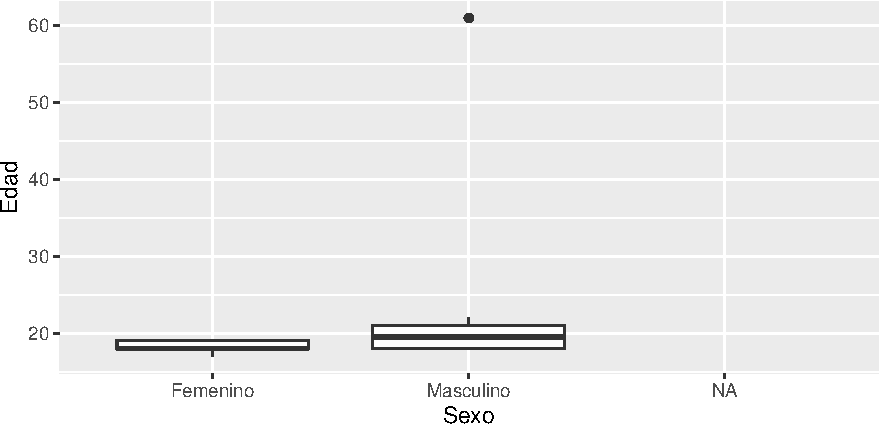
\includegraphics[width=0.8\linewidth,height=\textheight,keepaspectratio]{DatosEstaturaPeso_files/figure-beamer/unnamed-chunk-13-1.pdf}
\end{center}
\end{frame}

\begin{frame}[fragile]{Boxplot de edad por sexo}
\phantomsection\label{boxplot-de-edad-por-sexo-1}
Sin el dato atípico

\begin{Shaded}
\begin{Highlighting}[]
\NormalTok{datosn}\OtherTok{\textless{}{-}}\NormalTok{datos}\SpecialCharTok{|\textgreater{}}\FunctionTok{filter}\NormalTok{(Edad}\SpecialCharTok{\textless{}}\DecValTok{60}\NormalTok{)}

\FunctionTok{ggplot}\NormalTok{(}\AttributeTok{data=}\NormalTok{datosn,}\FunctionTok{aes}\NormalTok{(}\AttributeTok{x=}\NormalTok{Sexo,}\AttributeTok{y=}\NormalTok{Edad)) }\SpecialCharTok{+} \FunctionTok{geom\_boxplot}\NormalTok{() }
\end{Highlighting}
\end{Shaded}

\begin{center}
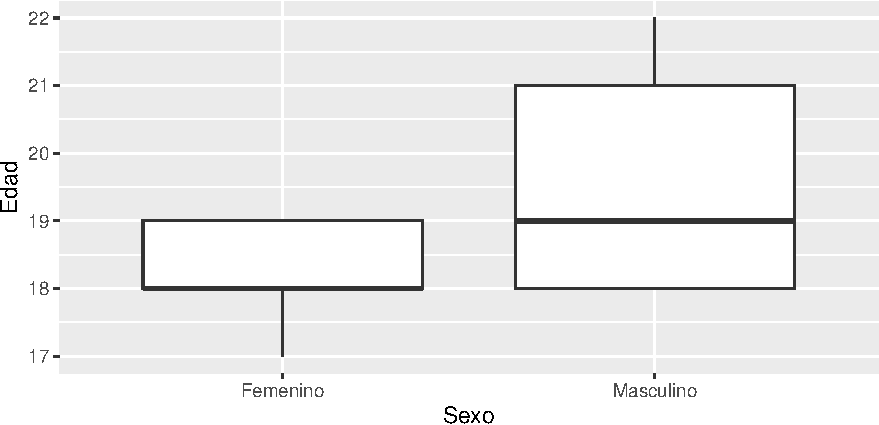
\includegraphics[width=0.8\linewidth,height=\textheight,keepaspectratio]{DatosEstaturaPeso_files/figure-beamer/unnamed-chunk-14-1.pdf}
\end{center}
\end{frame}

\begin{frame}[fragile]{Relación peso y estatura}
\phantomsection\label{relaciuxf3n-peso-y-estatura}
\begin{Shaded}
\begin{Highlighting}[]
\FunctionTok{ggplot}\NormalTok{(}\AttributeTok{data=}\NormalTok{datos,}\FunctionTok{aes}\NormalTok{(}\AttributeTok{x=}\NormalTok{Estatura,}\AttributeTok{y=}\NormalTok{peso)) }\SpecialCharTok{+} \FunctionTok{geom\_point}\NormalTok{() }
\end{Highlighting}
\end{Shaded}

\begin{center}
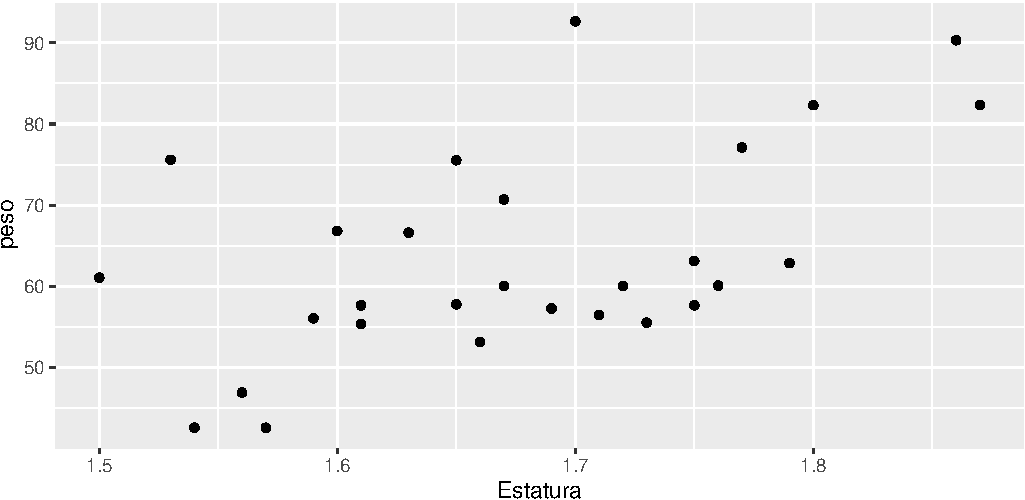
\includegraphics[width=0.95\linewidth,height=\textheight,keepaspectratio]{DatosEstaturaPeso_files/figure-beamer/unnamed-chunk-15-1.pdf}
\end{center}
\end{frame}

\begin{frame}[fragile]{Puntos con linea de regresión}
\phantomsection\label{puntos-con-linea-de-regresiuxf3n}
\begin{Shaded}
\begin{Highlighting}[]
\FunctionTok{ggplot}\NormalTok{(}\AttributeTok{data=}\NormalTok{datos,}\FunctionTok{aes}\NormalTok{(}\AttributeTok{x=}\NormalTok{Estatura,}\AttributeTok{y=}\NormalTok{peso)) }\SpecialCharTok{+} 
  \FunctionTok{geom\_point}\NormalTok{() }\SpecialCharTok{+} 
  \FunctionTok{geom\_smooth}\NormalTok{(}\AttributeTok{method =} \StringTok{"lm"}\NormalTok{,}\AttributeTok{se=}\ConstantTok{FALSE}\NormalTok{) }
\end{Highlighting}
\end{Shaded}

\begin{center}
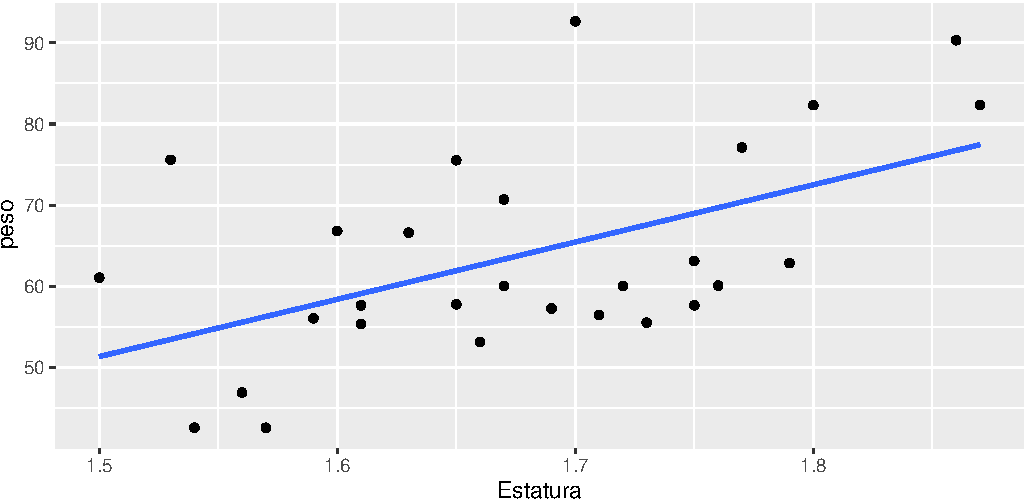
\includegraphics[width=0.9\linewidth,height=\textheight,keepaspectratio]{DatosEstaturaPeso_files/figure-beamer/unnamed-chunk-16-1.pdf}
\end{center}
\end{frame}

\begin{frame}[fragile]{Puntos diferenciados por sexo}
\phantomsection\label{puntos-diferenciados-por-sexo}
\begin{Shaded}
\begin{Highlighting}[]
\FunctionTok{ggplot}\NormalTok{(}\AttributeTok{data=}\NormalTok{datos,}\FunctionTok{aes}\NormalTok{(}\AttributeTok{x=}\NormalTok{Estatura,}\AttributeTok{y=}\NormalTok{peso)) }\SpecialCharTok{+}
  \FunctionTok{geom\_point}\NormalTok{(}\FunctionTok{aes}\NormalTok{(}\AttributeTok{col=}\NormalTok{Sexo)) }\SpecialCharTok{+} 
  \FunctionTok{geom\_smooth}\NormalTok{(}\AttributeTok{method =} \StringTok{"lm"}\NormalTok{,}\AttributeTok{se=}\ConstantTok{FALSE}\NormalTok{) }
\end{Highlighting}
\end{Shaded}

\begin{center}
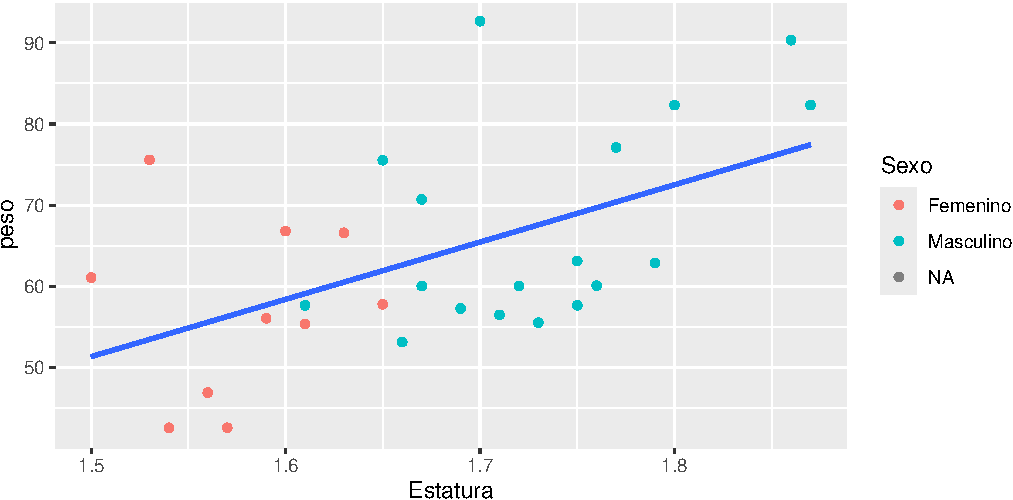
\includegraphics[width=0.9\linewidth,height=\textheight,keepaspectratio]{DatosEstaturaPeso_files/figure-beamer/unnamed-chunk-17-1.pdf}
\end{center}
\end{frame}




\end{document}
